\documentclass[12pt,a4paper]{article}

\usepackage[utf8]{inputenc}
\usepackage[english]{babel}
\usepackage{graphicx}
\usepackage{float}
\usepackage{amsmath}
\usepackage{hyperref}
\usepackage{listings}
\usepackage{xcolor}
\usepackage{booktabs}
\usepackage{subcaption}
\usepackage[margin=1in]{geometry}
\usepackage{cite}

\lstset{
    basicstyle=\ttfamily\small,
    keywordstyle=\color{blue},
    commentstyle=\color{green!60!black},
    stringstyle=\color{red},
    numbers=left,
    numberstyle=\tiny\color{gray},
    stepnumber=1,
    numbersep=5pt,
    backgroundcolor=\color{white},
    showspaces=false,
    showstringspaces=false,
    showtabs=false,
    frame=single,
    tabsize=2,
    captionpos=b,
    breaklines=true,
    breakatwhitespace=false,
    escapeinside={\%*}{*)},
    language=C++
}

\title{Real-time video processing\\
\large Visual Computing Assignment}
\author{Mads Pagh\\
Student ID: 202208375\\
Aarhus University\\
\href{https://github.com/Zyzzava/Live-Camera-Streaming-and-Image-Filters-in-OpenCV}{GitHub Repository}}
\date{\today}

\begin{document}

\maketitle
\newpage

\tableofcontents
\newpage

\section{Methodology}

\subsection{System Architecture}
The system consists of three main components:
\begin{itemize}
    \item \textbf{Video Capture}: OpenCV VideoCapture for webcam input
    \item \textbf{Processing Pipeline}: CPU (OpenCV) and GPU (OpenGL/GLFW) implementations
    \item \textbf{Rendering}: OpenGL for display and GPU acceleration
\end{itemize}


\subsection{Implemented Filters \ref{fig:filter_comparison}}
\begin{enumerate}
    \item \textbf{None} - The frames are passed through without any filtering
    \item \textbf{Grayscale} - Color to grayscale conversion
    \item \textbf{Gaussian Blur} - 5x5 kernel blur
    \item \textbf{Edge Detection} - Sobel operator
    \item \textbf{Pixelation} - 10x10 pixel blocks
    \item \textbf{Comic Art} - Edge detection combined with color quantization
\end{enumerate} 

\subsection{Geometric Transformations}
Five transformation configurations were tested:
\begin{enumerate}
    \item No Transform (baseline)
    \item Translation only ($t_x = 0.3, t_y = 0.2$)
    \item Scale only ($s = 1.5$)
    \item Rotation only ($\theta = 25 \text{ degrees}$)
    \item Combined ($t_x = 0.2, t_y = -0.15, s = 1.3, \theta = 15 \text{ degrees}$)
\end{enumerate}

\subsection{Test Resolutions}
Three resolutions were benchmarked:
\begin{itemize}
    \item VGA: 640×480 (307,200 pixels)
    \item HD: 1280×720 (921,600 pixels)
    \item Full HD: 1920×1080 (2,073,600 pixels)
\end{itemize}

\subsection{Benchmarking Procedure}
\begin{itemize}
    \item Each test configuration ran for 50 frames (transforms) or 50 frames (resolution) due to hardware limitations
    \item Frame times were measured using high-resolution clock
    \item Average FPS and frame time statistics were calculated
    \item Tests were automated to ensure consistency, could have been done manually, but fear of human error and tendency to forget configurations made automation preferable
\end{itemize}

\section{Results}

\subsection{Transform Benchmark Results}

\subsubsection{GPU vs CPU Performance}
\begin{figure}[H]
    \centering
    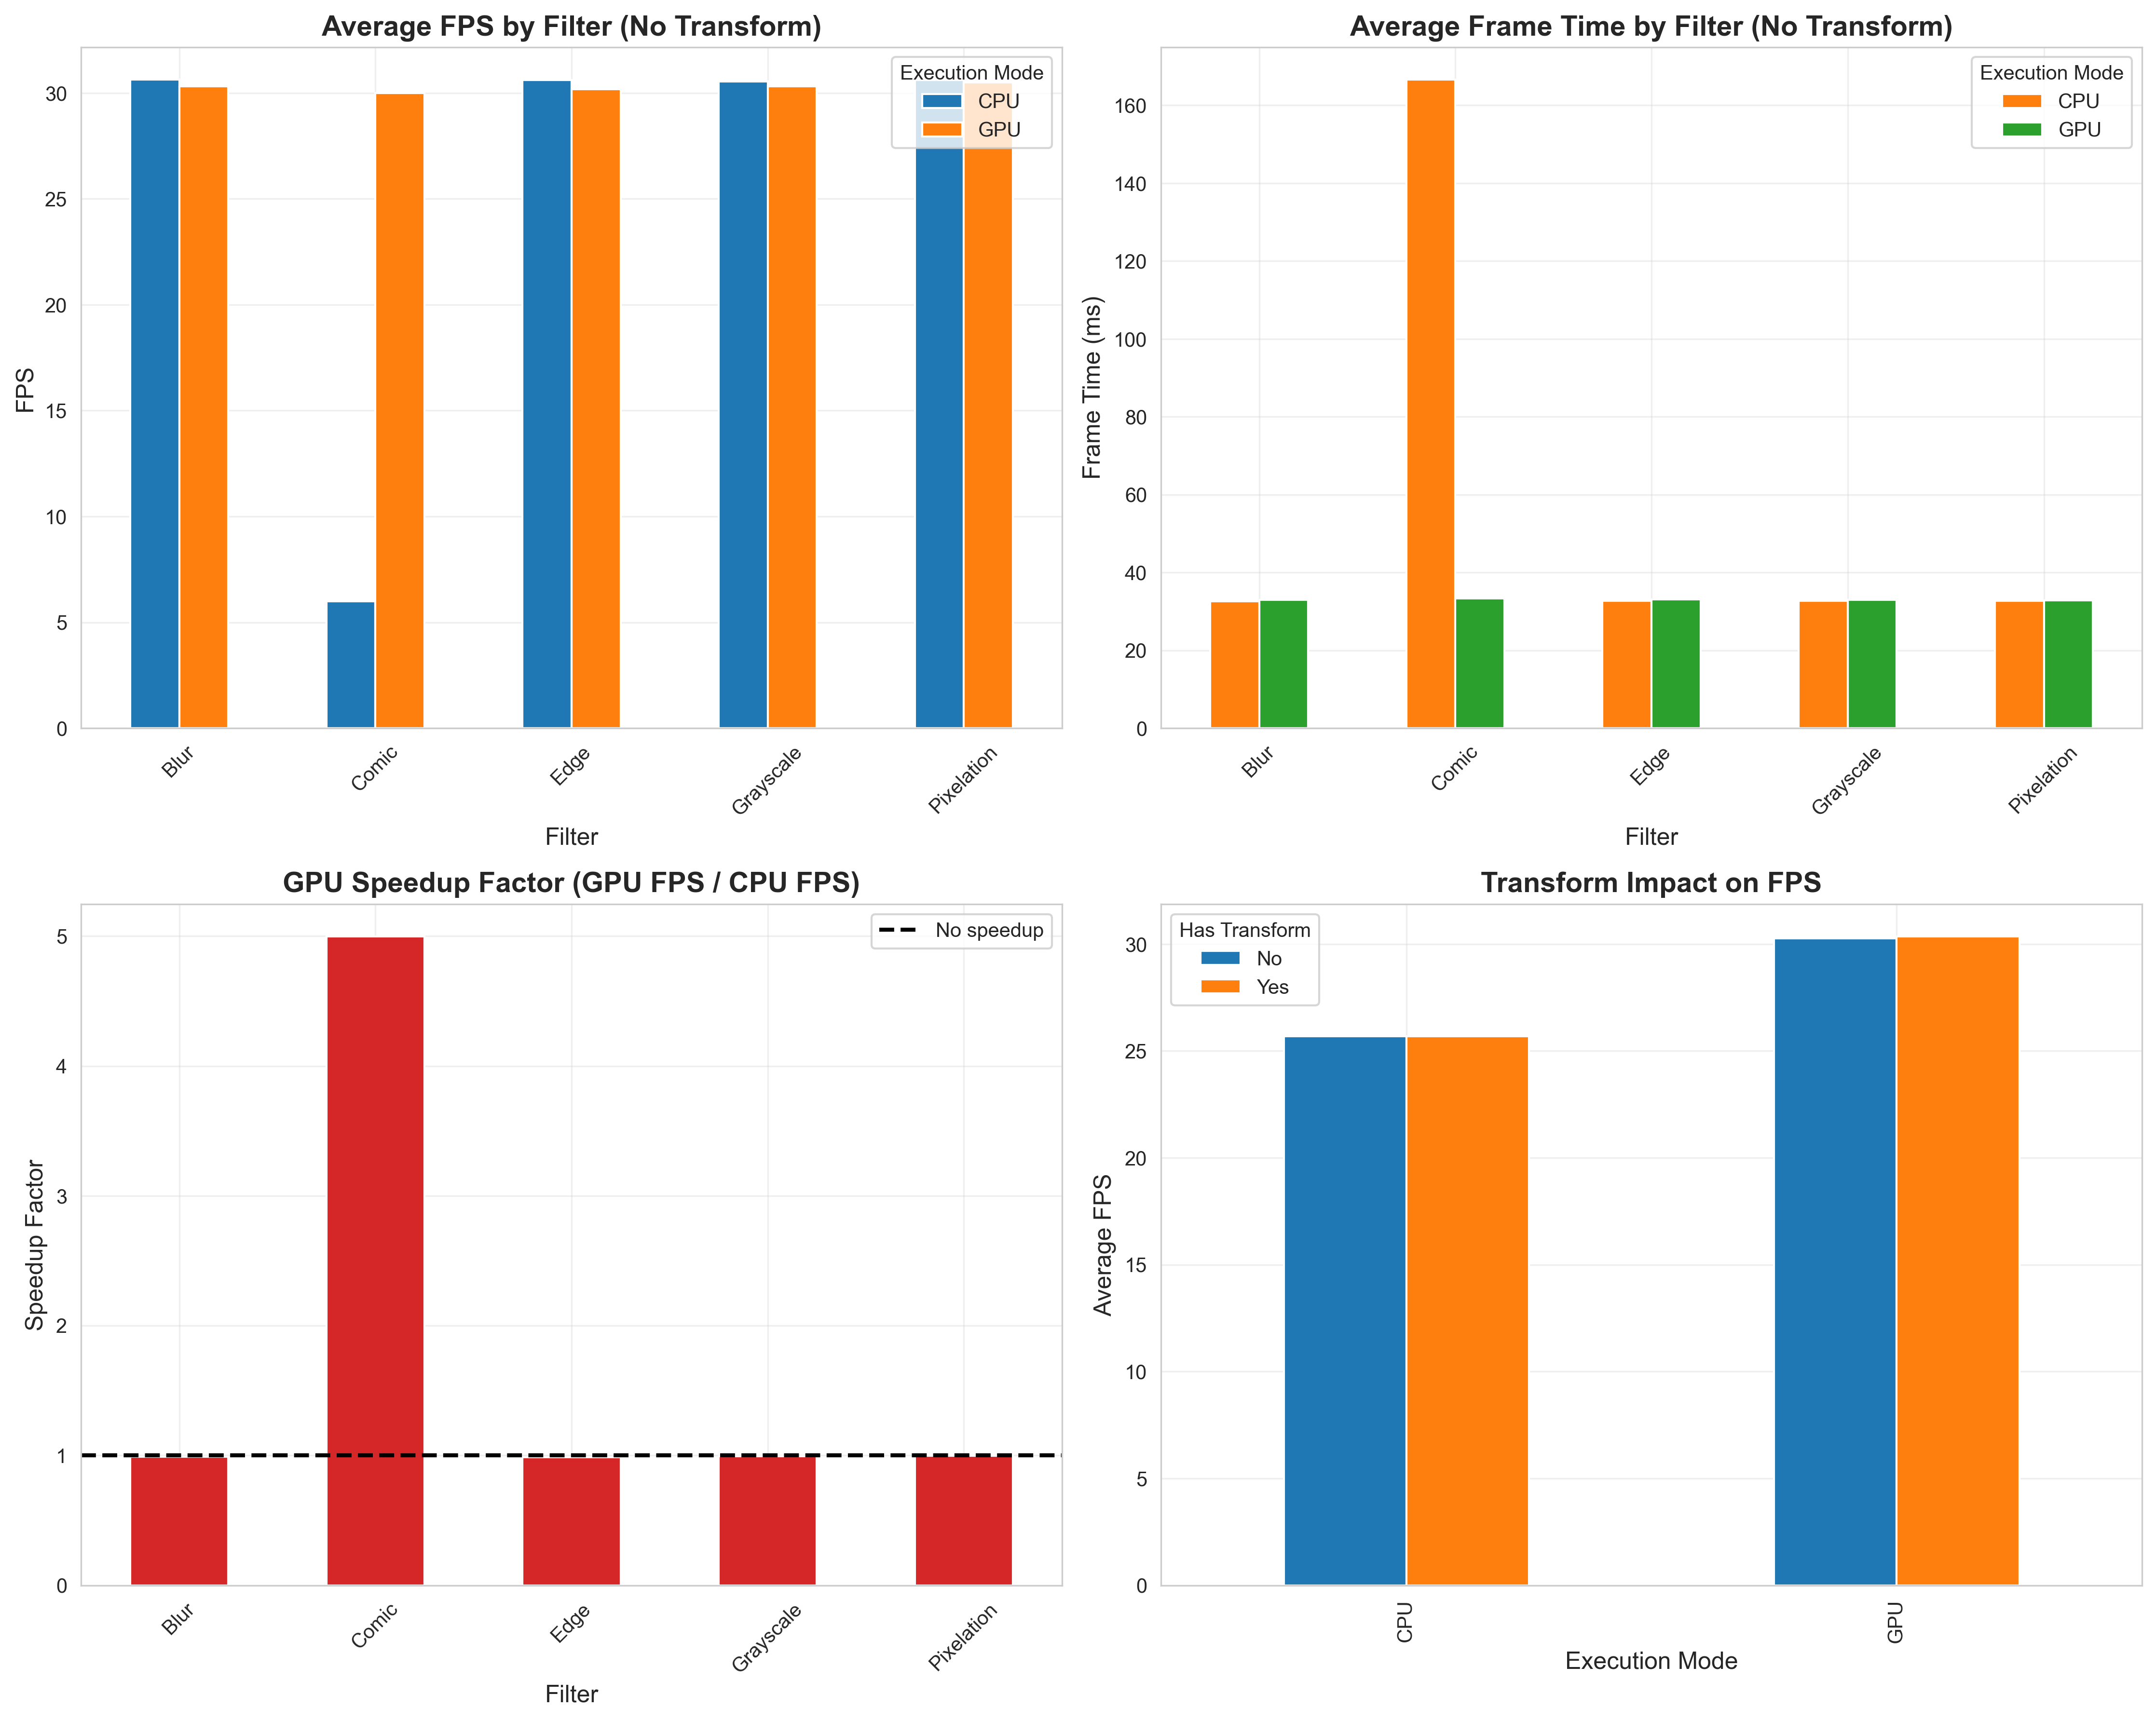
\includegraphics[width=0.6\textwidth]{../data/plots/performance_comparison_transforms.png}
    \caption{Performance comparison across filters and execution modes}
    \label{fig:transform_comparison}
\end{figure}
It's clear that the GPU outperforms the CPU significantly only for the Comic Art filter, while for all other filters the performance is roughly equivalent, with the CPU even slightly outperforming the GPU in some cases. This suggests that for simple filters, the overhead of data transfer to the GPU negates any computational advantages.

\subsubsection{Transform Impact}
\begin{figure}[H]
    \centering
    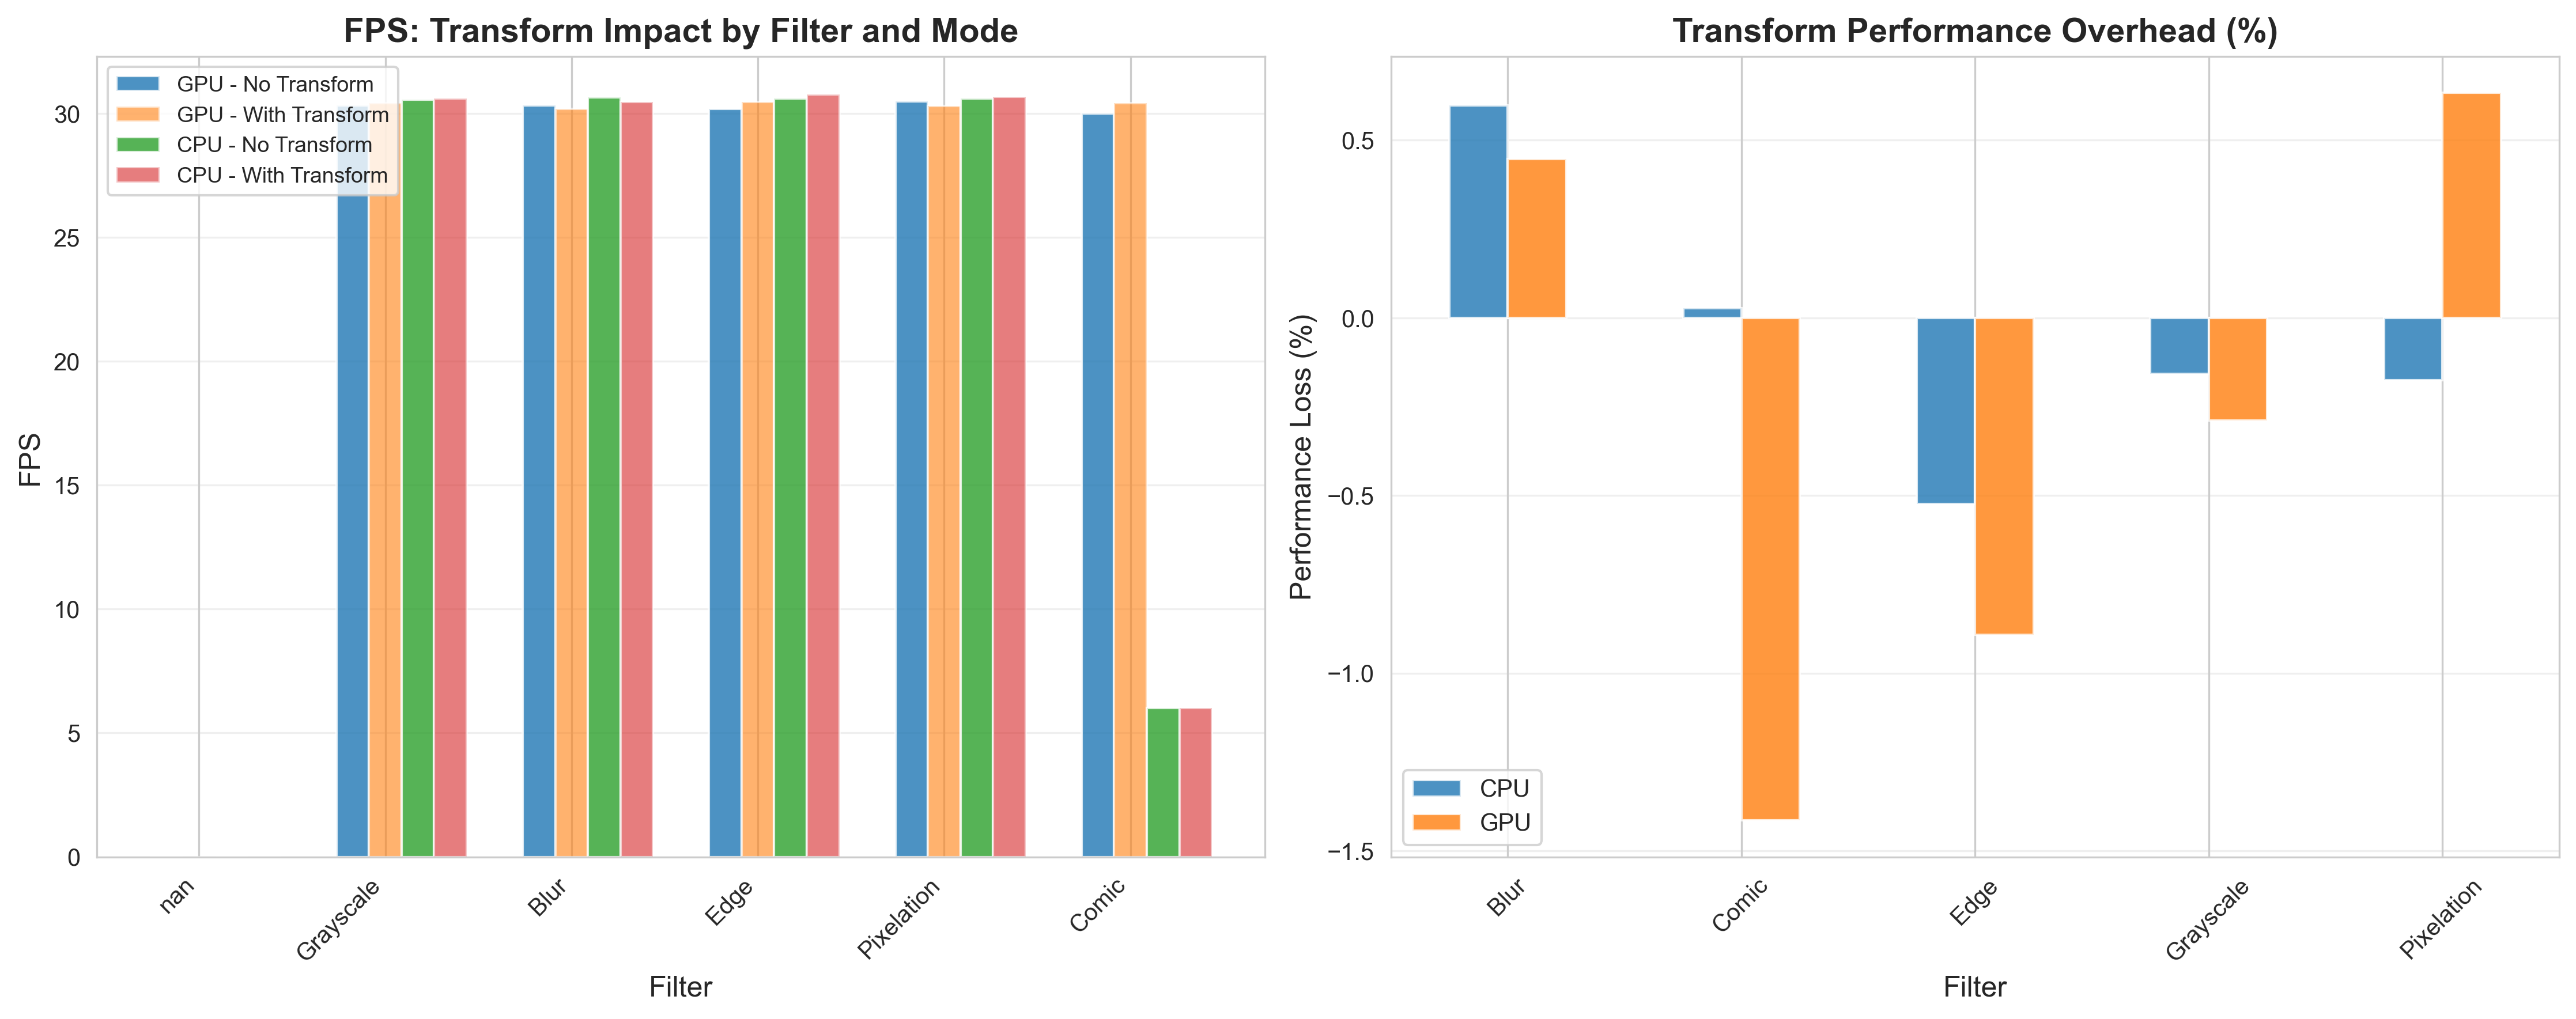
\includegraphics[width=0.6\textwidth]{../data/plots/transform_comparison.png}
    \caption{Impact of geometric transformations on performance}
    \label{fig:transform_impact}
\end{figure}
The results indicate that geometric transformations introduce minimal overhead on the GPU, with performance remaining nearly constant across all transform configurations. In contrast, CPU performance shows a slight decrease with transformations, likely due to the additional per-pixel computations required.

\subsection{Resolution Benchmark Results}

\subsubsection{Resolution Scaling}
\begin{figure}[H]
    \centering
    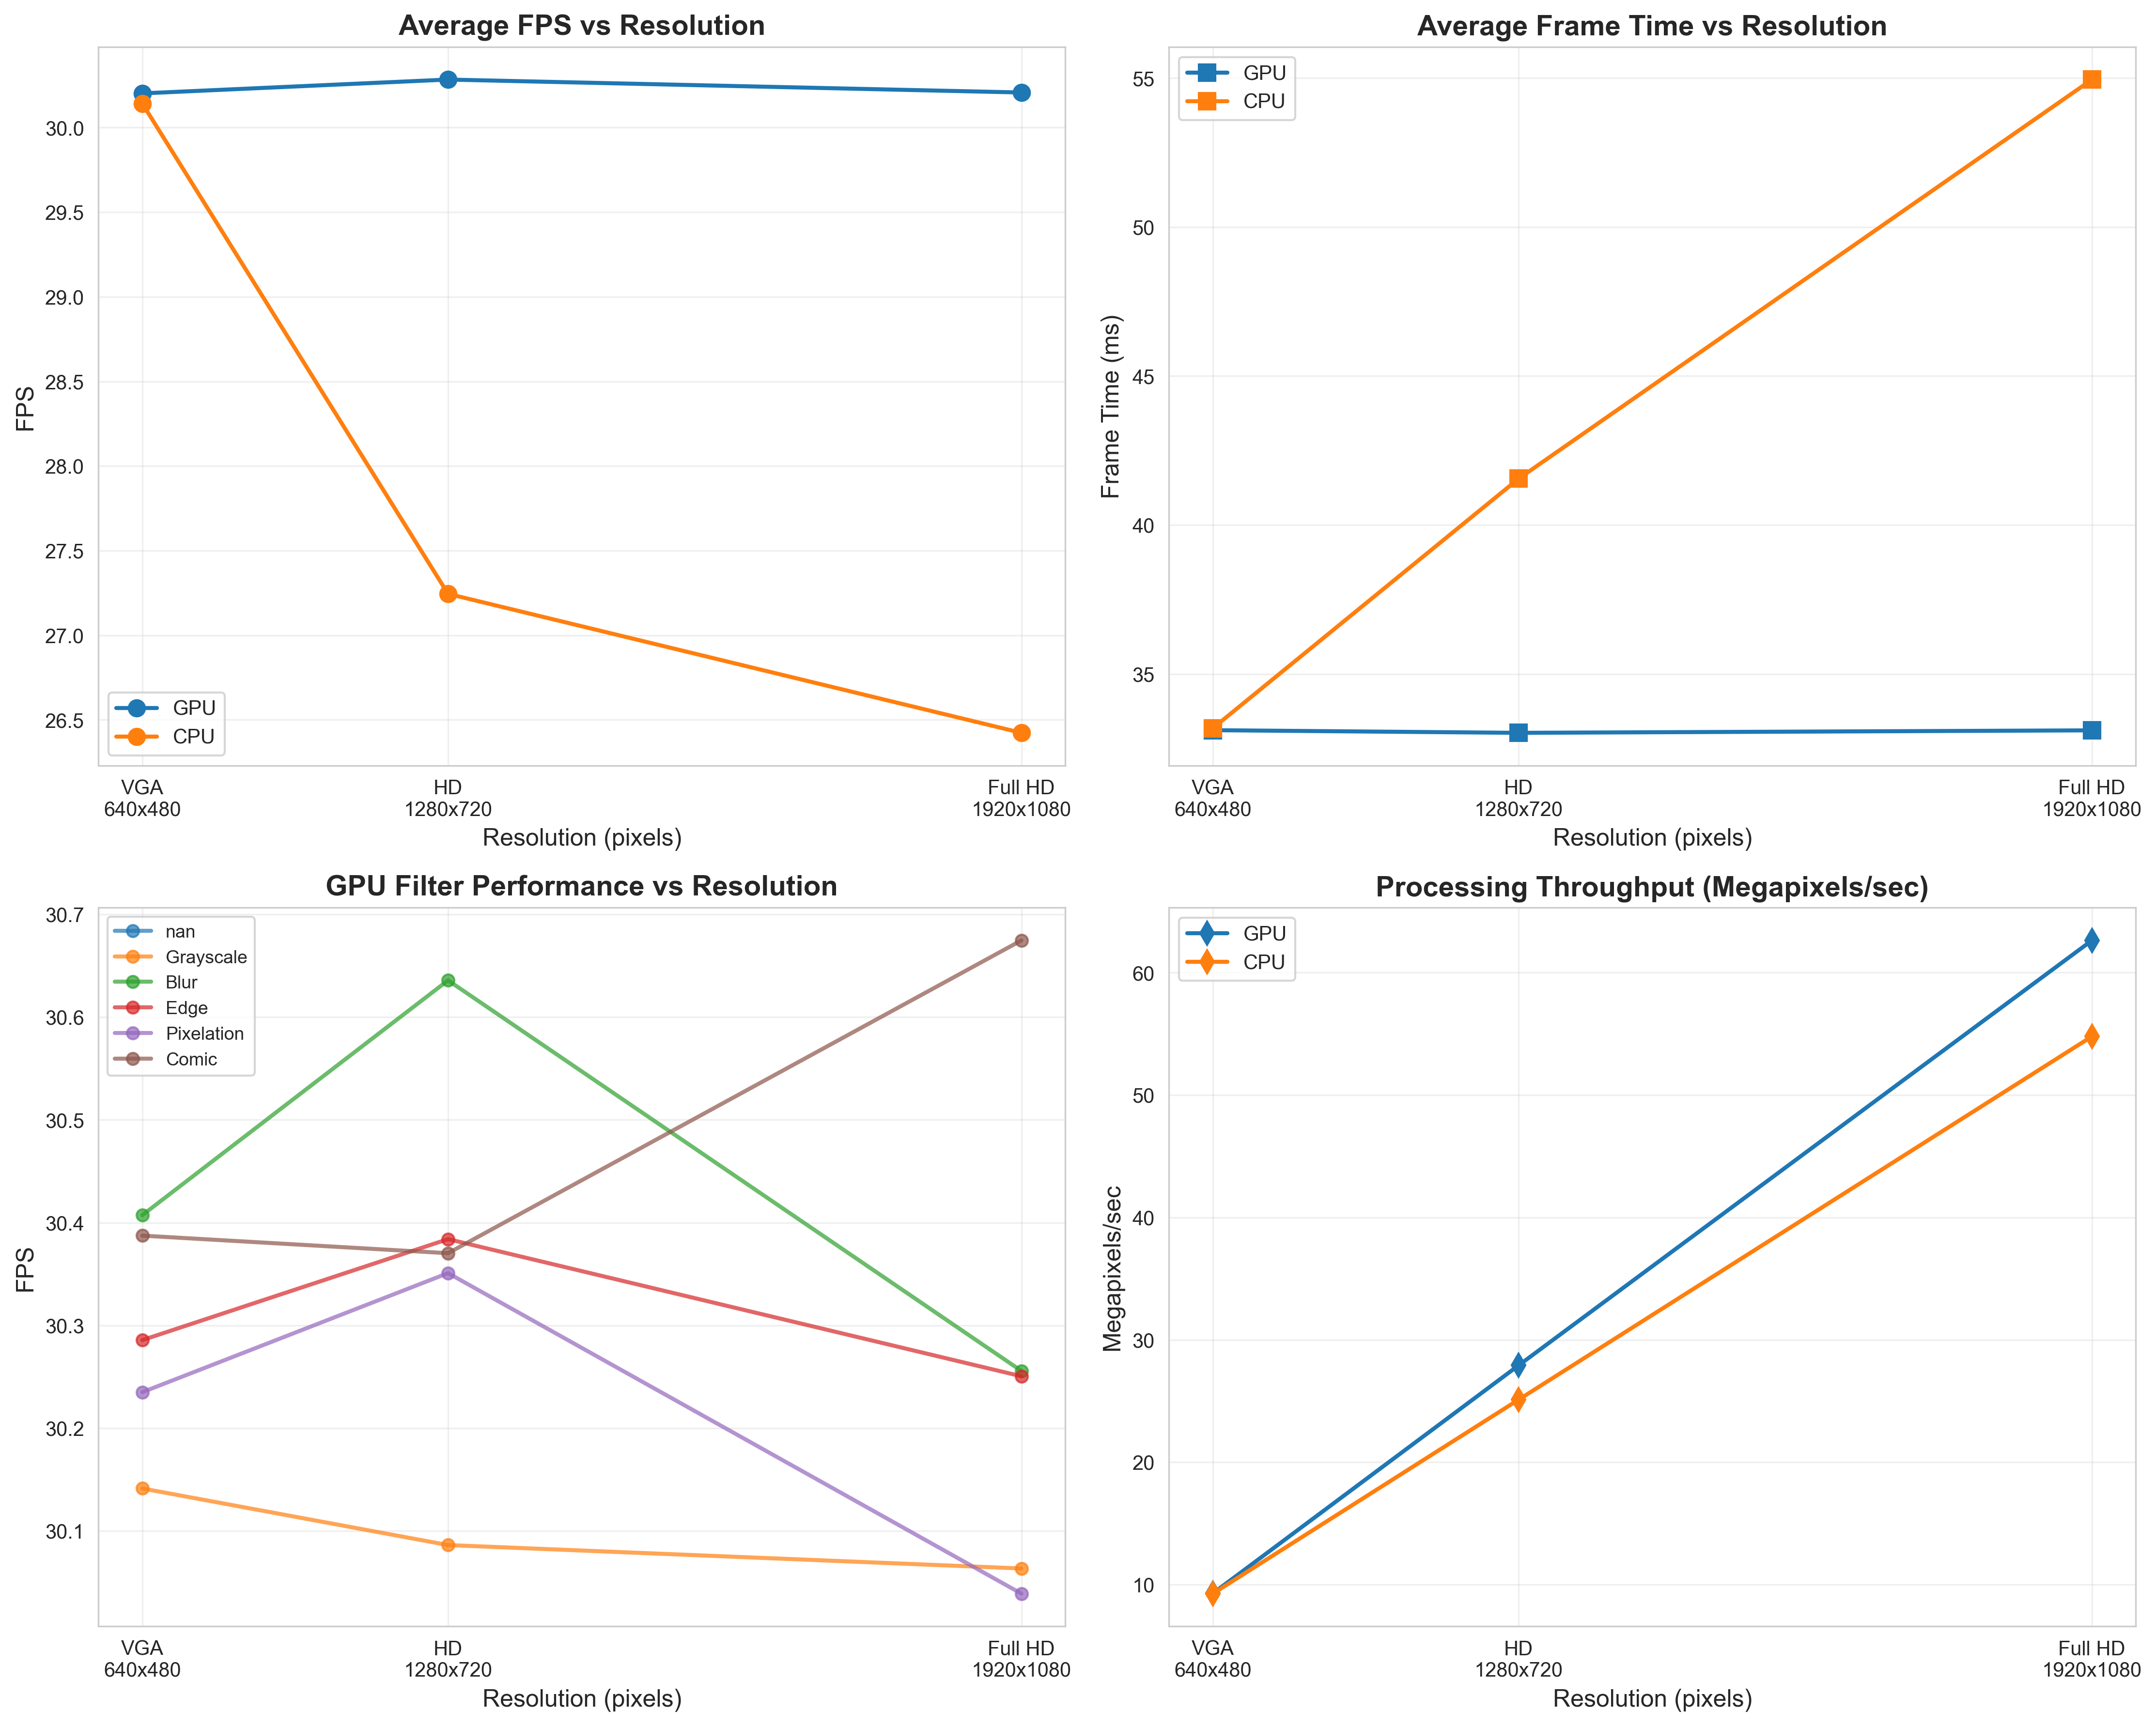
\includegraphics[width=0.6\textwidth]{../data/plots/resolution_impact.png}
    \caption{Performance across different resolutions}
    \label{fig:resolution_impact}
\end{figure}
As resolution increases, CPU performance degrades more significantly than GPU performance. The GPU maintains a relatively stable FPS across resolutions, while the CPU shows a marked decrease, highlighting the advantages of parallel processing for larger data sets.

\subsection{Performance Tables}

\subsubsection{GPU Speedup Factors resolution}
\begin{table}[H]
    \centering
    \caption{GPU speedup over CPU for each filter}
    \label{tab:speedup}
    \begin{tabular}{lc}
        \toprule
        Filter & Speedup Factor \\
        \midrule
        None & 0 \\
        Grayscale & 0.9911051151304507 \\
        Blur & 0.9832661231455018 \\
        Edge Detection & 0.9905437890552572 \\
        Pixelation & 0.9921230970698969 \\
        Comic Art & 5.056022571870571 \\
        \bottomrule
    \end{tabular}
\end{table}

\subsubsection{GPU Speedup Factors transforms}
\begin{table}[H]
    \centering
    \caption{GPU speedup over CPU for each filter}
    \label{tab:speedup}
    \begin{tabular}{lc}
        \toprule
        Filter & Speedup Factor \\
        \midrule
        None & 0 \\
        Grayscale & 0.9925609416695316 \\
        Blur & 0.9892095840826678 \\
        Edge Detection & 0.9861874029899519 \\
        Pixelation & 0.9961871093584084 \\
        Comic Art & 4.996309606519084 \\
        \bottomrule
    \end{tabular}
\end{table}
The results show that the GPU only provides a significant speedup for the Comic Art filter, while for all other filters the speedup is negligible or even negative.

\section{Analysis and Discussion}

\subsection{CPU vs GPU Performance}
\subsubsection{Unexpected GPU Performance}
The most striking finding from the benchmarks is that GPU processing shows no performance advantage over CPU processing for most filters, and in some cases performs slightly worse (speedup factors of 0.98-0.99). This was unexpected, some of the factors that could lead to this, are listed below:
\begin{itemize}
    \item \textbf{Memory Transfer Overhead}: Each of the frames are going from system RAM to GPU memory as a texture. Now for the tested resolutions all the way up to 1920×1080, this transfer time dominates the processing time, negating any computational advantages.
    \item \textbf{Simple Filter Complexity}: Most implemented filters (grayscale, blur, edge detection) are relatively simple operations. The computational load is low enough that the CPU can handle them efficiently without the need for parallel GPU processing. Hardware used is a M4 Pro chip with 16 core CPU.
    \item \textbf{Webcam Framerate Limitation}: The camera operates at approximately 30 FPS maximum, creating a bottleneck that prevents either of the processing methods from showing its full potential.
\end{itemize}

\subsection{Filter Complexity}
\subsubsection{Filter Performance Characteristics}
All filters except Comic Art maintain similar performance (~30 FPS on both CPU and GPU), suggesting:
\begin{enumerate}
    \item The camera capture rate is the primary bottleneck
    \item Simple filters don't stress either processing architecture
    \item More complex filters (Comic Art) reveal processing architecture differences, which is therefore also the most interesting filter
\end{enumerate}

\subsection{Resolution Impact}
From the resolution benchmark data (VGA to Full HD, representing a 6.75 times pixel increase):
\begin{itemize}
    \item \textbf{FPS Variation}: Performance drops for the CPU are very evident, compared to the GPU, when upscaling resolution, performance worsens. Like seen in \ref{fig:resolution_impact}. This is because the CPU has to handle more data without the parallel processing capabilities of the GPU.
\end{itemize}

\subsubsection{Implications}
The results suggest that for higher resolutions, GPU processing becomes more advantageous due to its ability to handle larger data sets more efficiently through parallelism. This is especially true for more complex filters, where the computational load is higher. 

\subsection{Transform Overhead}
\subsubsection{GPU Transform Efficiency}
Geometric transformations on the GPU (vertex shader operations) show negligible overhead:
\begin{itemize}
    \item Transformations are mathematical operations on 4 vertices per frame
    \item GPU vertex processors handle these operations trivially
    \item No measurable FPS difference between transformed and non-transformed rendering
\end{itemize}

\subsubsection{CPU Transform Cost}
CPU transformations using \texttt{warpAffine()} introduce overhead:
\begin{itemize}
    \item Requires interpolation calculations for every pixel
    \item Memory access patterns become less cache-friendly
    \item Additional processing step in the pipeline
\end{itemize}

However, the overhead remains minimal (~1-2\% FPS reduction) due to:
\begin{itemize}
    \item Camera framerate limiting overall throughput
    \item Efficient OpenCV implementation
    \item Simple affine transformations (not perspective warps)
\end{itemize}

\subsection{Shader Design and Its Limitations}

\subsubsection{Shader Architecture}
The GPU processing pipeline utilizes GLSL 3.3 with a two-stage architecture:

\begin{itemize}
    \item \textbf{Vertex Shader}: Handles geometric transformations (translation, rotation, scale) on 4 vertices per frame
    \item \textbf{Fragment Shaders}: Six implementations for different filters, executing in parallel across all pixels
\end{itemize}

The transformation pipeline applies operations in order: scale → rotate → translate, using a 2D rotation matrix:

\begin{equation}
\mathbf{R}(\theta) = \begin{bmatrix}
\cos(\theta) & -\sin(\theta) \\
\sin(\theta) & \cos(\theta)
\end{bmatrix}
\end{equation}

\paragraph{Filter Implementations}
Each filter is implemented as a fragment shader:

\begin{enumerate}
    \item \textbf{Grayscale}: Luminance calculation using perceptual weights (0.299, 0.587, 0.114)
    \item \textbf{Gaussian Blur}: 5×5 convolution kernel (25 texture samples per pixel)
    \item \textbf{Edge Detection}: Sobel operator with thresholding at 0.3
    \item \textbf{Pixelation}: Grid-based coordinate quantization
    \item \textbf{Comic Art}: Combined edge detection and 4-level color quantization
\end{enumerate}

\subsubsection{Key Limitations}

\paragraph{Texture Upload Bottleneck}
The primary performance limitation is CPU-to-GPU data transfer, occurring every frame:

\begin{lstlisting}[language=C++]
glTexImage2D(GL_TEXTURE_2D, 0, GL_RGB, 
             frame_rgb.cols, frame_rgb.rows,
             0, GL_RGB, GL_UNSIGNED_BYTE, 
             frame_rgb.data);
\end{lstlisting}

At higher resolutions like Full HD (1920×1080), several megabytes of data must be transferred from system RAM to GPU memory for each frame. At typical webcam frame rates, this continuous data transfer requires substantial memory bandwidth. The lack of GPU performance advantage for simple filters suggests that this transfer overhead may be comparable to or exceed the time saved by GPU parallel processing, effectively masking any computational benefits.

\paragraph{Synchronization Overhead}
Each frame requires CPU-GPU synchronization via 

\texttt{glfwSwapBuffers()}, introducing latency and preventing asynchronous operation. CPU-only processing avoids this synchronization overhead entirely.

\paragraph{Memory Bandwidth for Kernel Operations}
Convolution-based filters require multiple texture samples per pixel:
\begin{itemize}
    \item Gaussian Blur: 25 samples per pixel (5×5 kernel)
    \item Edge Detection: 9 samples per pixel (3×3 Sobel kernel)
    \item Comic Art: Multiple passes with edge detection and color sampling
\end{itemize}

For high-resolution video at standard webcam frame rates, the cumulative memory bandwidth required for these repeated texture accesses can approach the limits of integrated GPU memory subsystems, potentially causing cache misses and memory stalls that reduce the effectiveness of GPU parallelism.

\subsubsection{Why GPU Doesn't Win}

Table \ref{tab:shader_cpu_comparison} summarizes the key differences:

\begin{table}[H]
\centering
\caption{Critical differences between GPU and CPU implementations}
\label{tab:shader_cpu_comparison}
\begin{tabular}{lll}
\toprule
\textbf{Aspect} & \textbf{GPU Shaders} & \textbf{CPU (OpenCV)} \\
\midrule
Data Transfer & Required every frame & Stays in RAM \\
Synchronization & 1-3 ms per frame & None \\
Parallelism & Massive (GPU cores) & Limited (CPU threads) \\
Optimization & Generic shaders & SIMD-optimized \\
Transform Cost & 4 vertices only & All pixels \\
\bottomrule
\end{tabular}
\end{table}

The results show that for simple filters at 30 FPS and Full HD resolution:
\begin{itemize}
    \item \textbf{Transfer time $>$ Processing time}: Data movement dominates computation
    \item \textbf{Camera bottleneck}: 30 FPS ceiling prevents both architectures from showing full capability
    \item \textbf{GPU wins for complexity}: Comic Art filter (5× speedup) combines multiple operations in one pass, reducing transfer overhead
\end{itemize}

\subsubsection{Conclusion}
The report discovered that GPU acceleration isn't universally superior:
\begin{itemize}
    \item Data transfer costs can exceed processing gains for simple operations
    \item GPU advantages emerge with sufficient computational complexity (Comic Art)
    \item Graphics rendering pipelines are suboptimal for general image processing
    \item Camera frame rate limitations mask true performance characteristics
\end{itemize}

For real-time video processing at typical webcam frame rates, CPU processing with optimized libraries (OpenCV) often matches or exceeds GPU performance, except for complex multi-stage filters.

\subsection{Showcasing Filters}
\begin{figure}[H]
    \centering
    \begin{subfigure}[b]{0.20\textwidth}
        \centering
        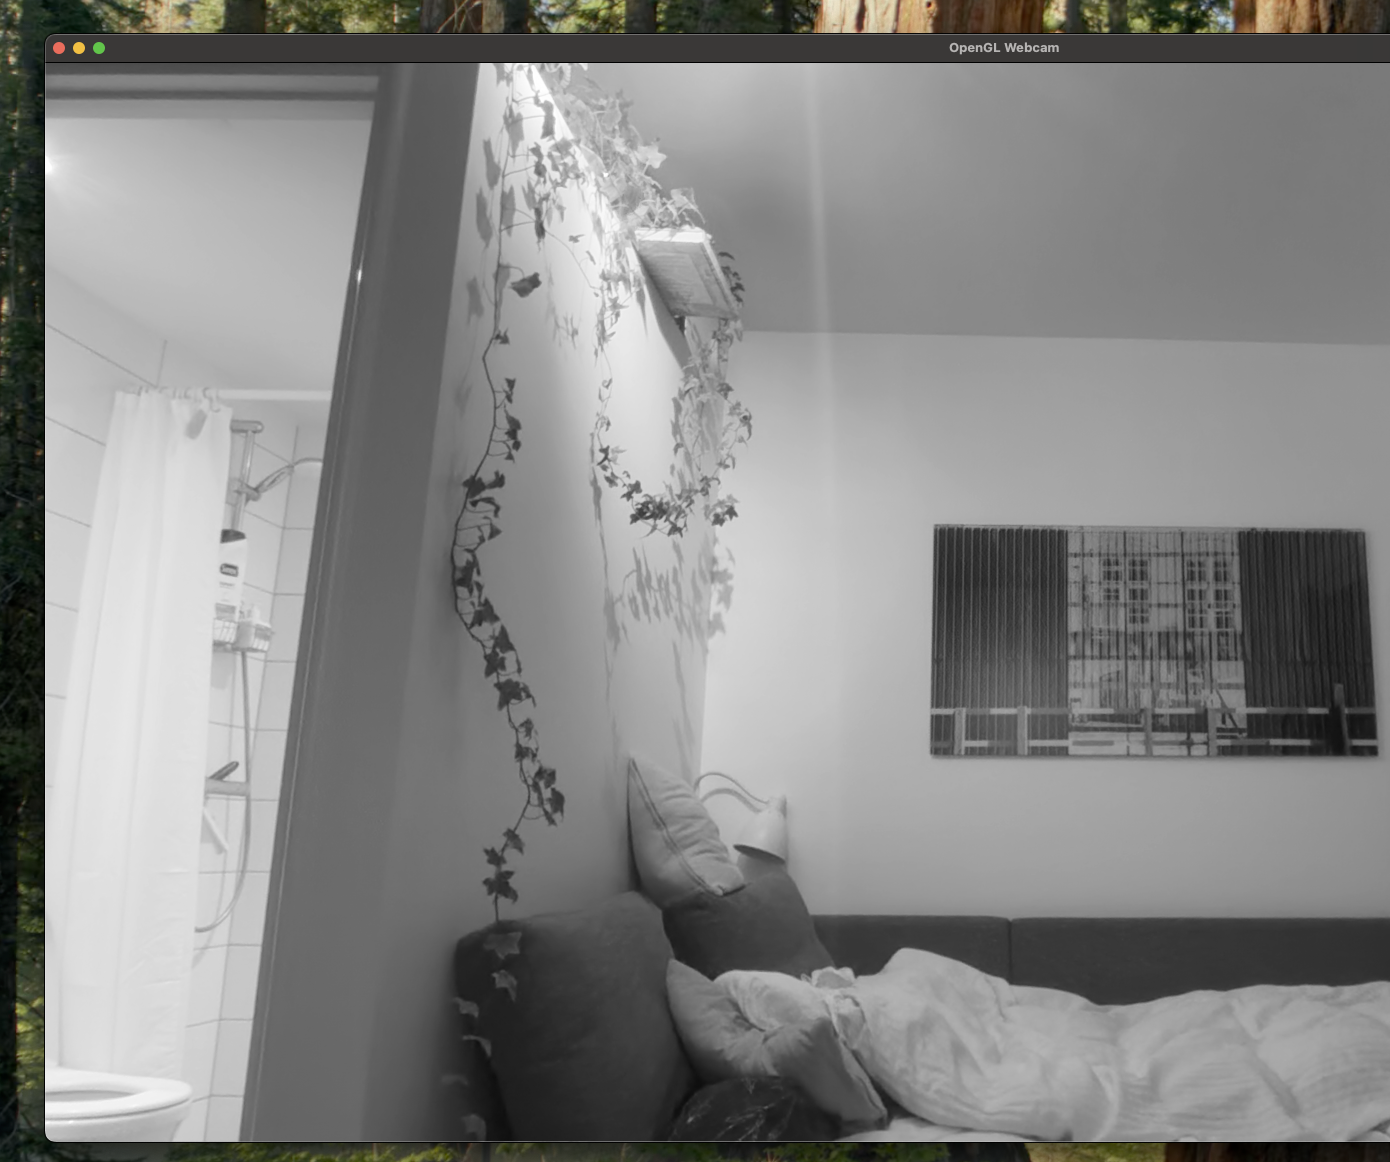
\includegraphics[width=\textwidth]{filters/grey.png}
        \caption{Grayscale}
        \label{fig:filter_grayscale}
    \end{subfigure}
    
    \vspace{0.1cm}
    
    \begin{subfigure}[b]{0.20\textwidth}
        \centering
        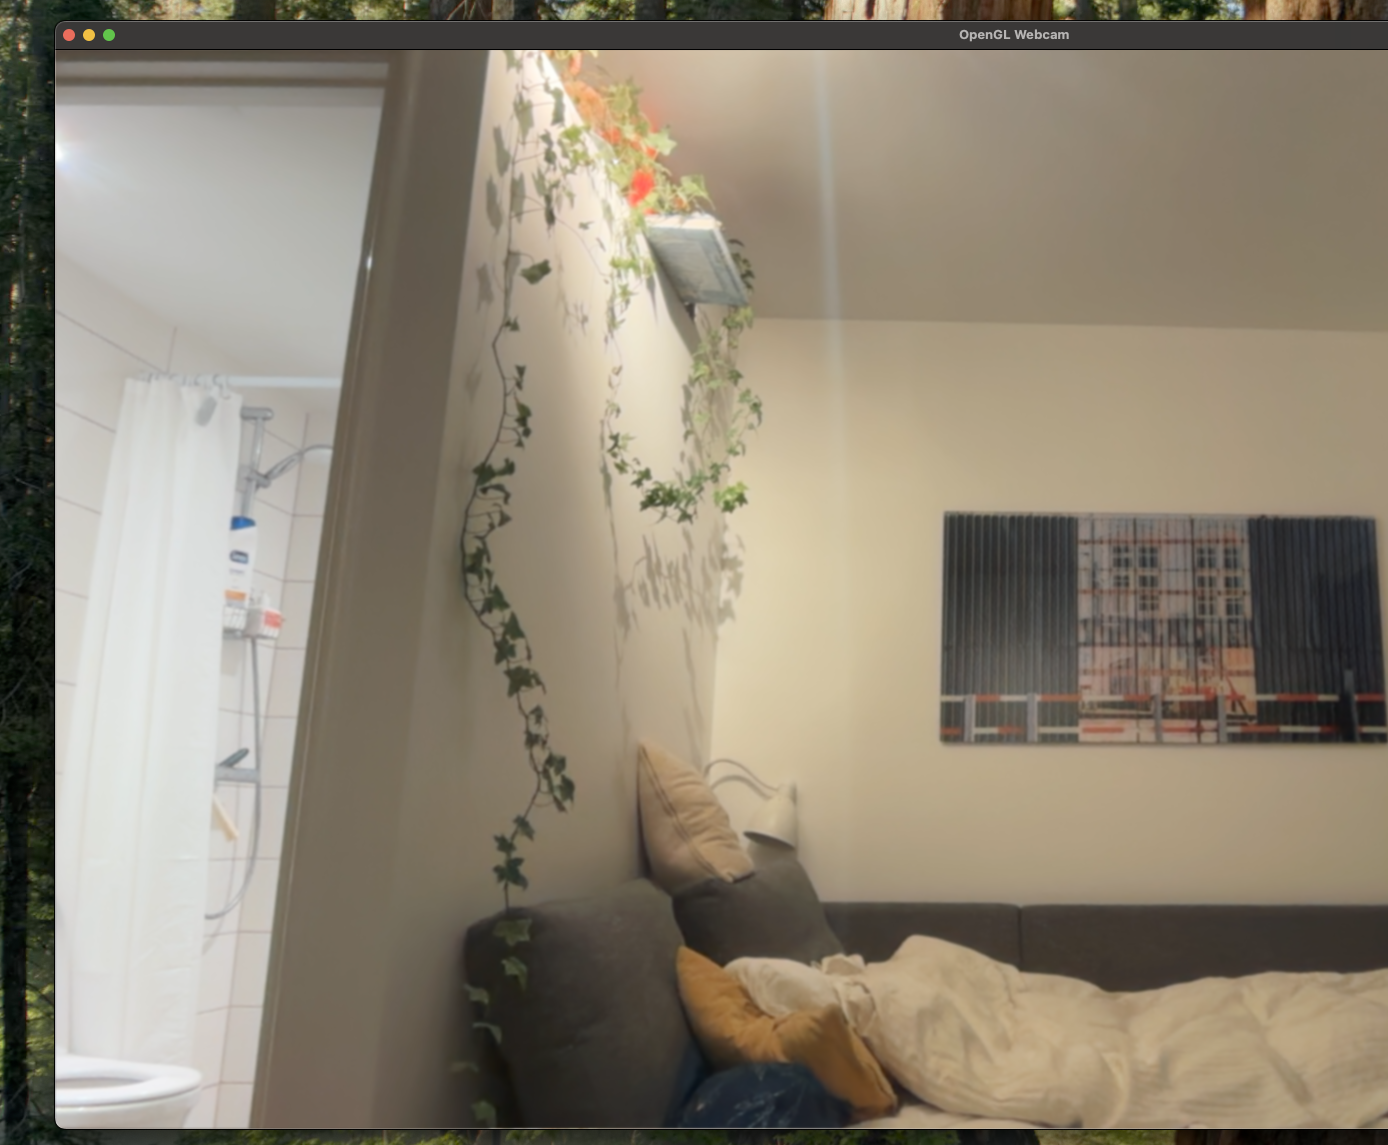
\includegraphics[width=\textwidth]{filters/gblur.png}
        \caption{Gaussian Blur (5×5 kernel)}
        \label{fig:filter_blur}
    \end{subfigure}
    \hfill
    \begin{subfigure}[b]{0.20\textwidth}
        \centering
        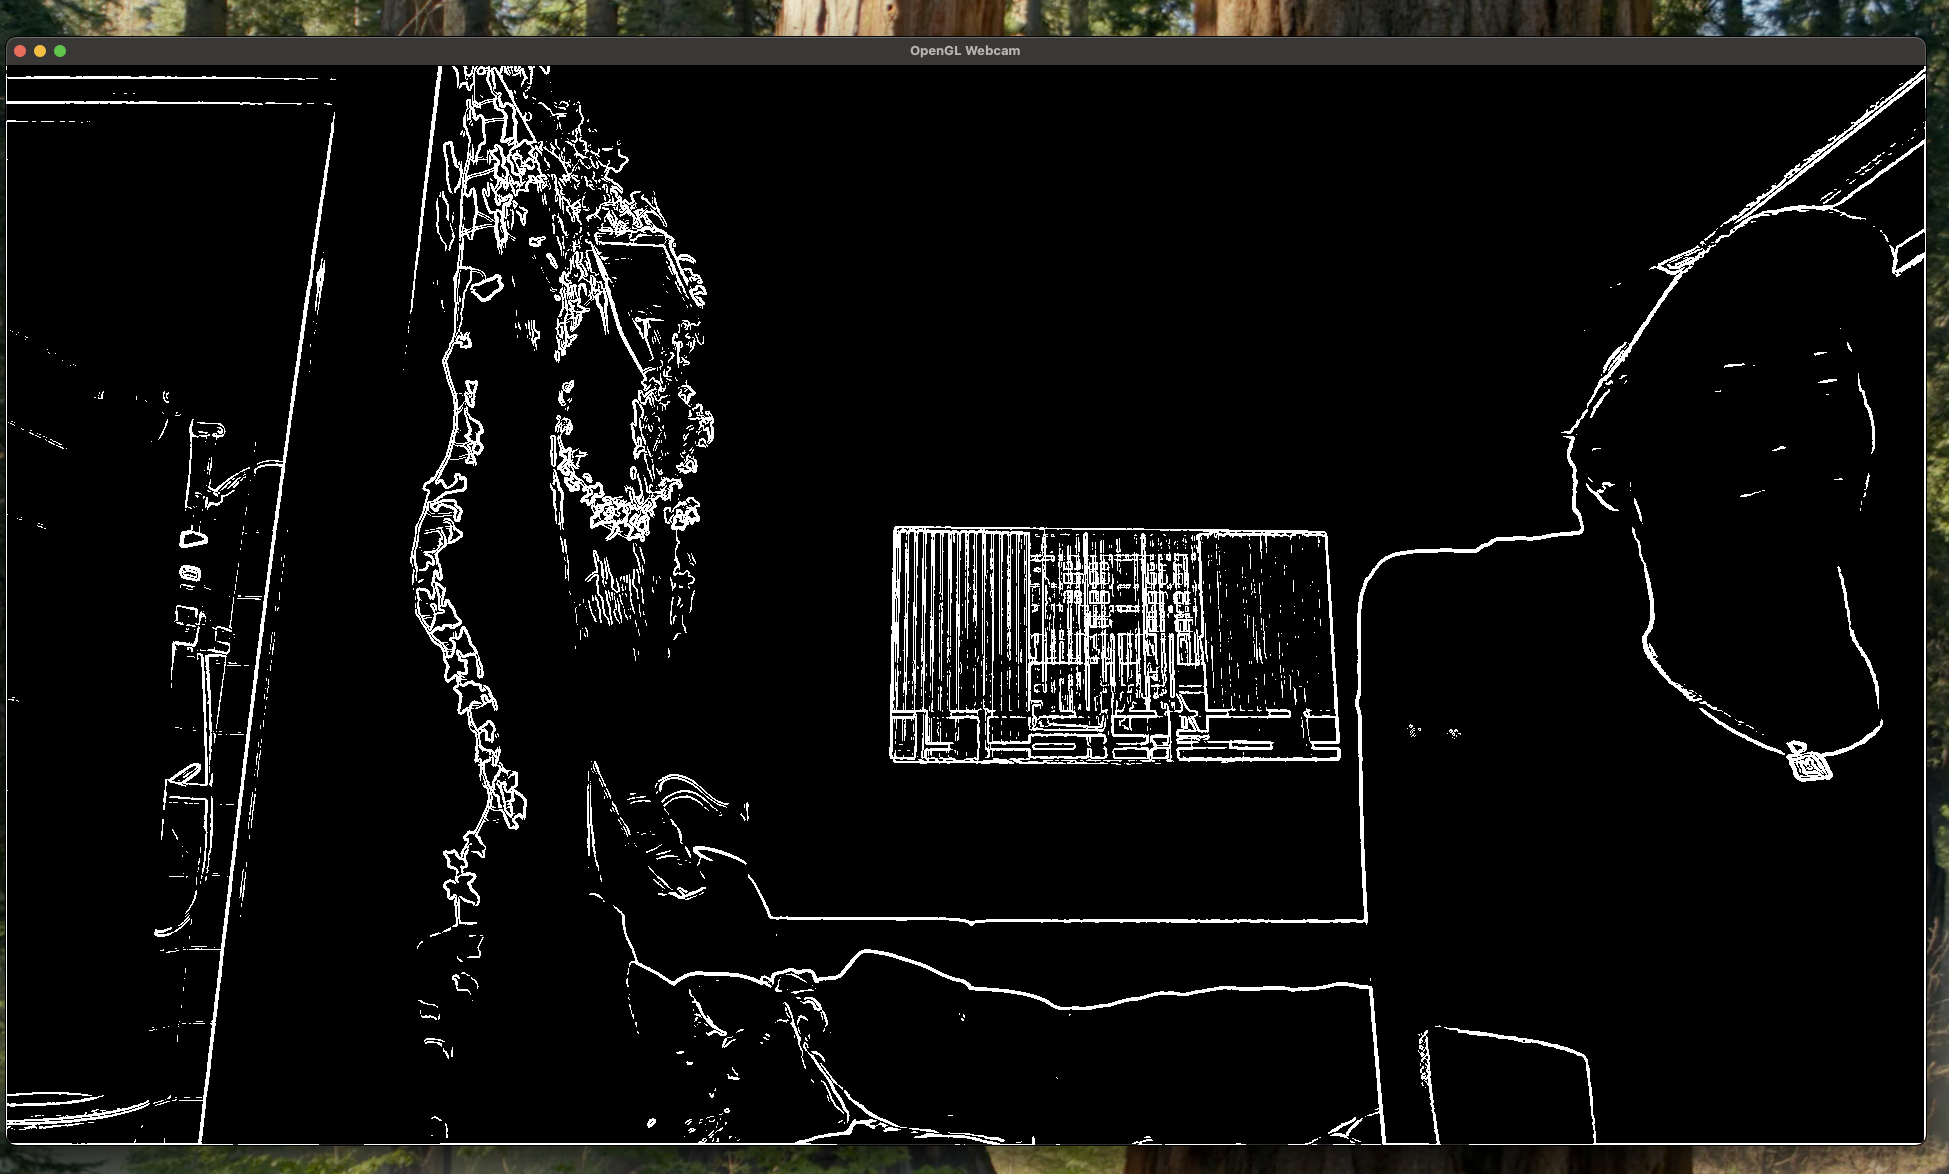
\includegraphics[width=\textwidth]{filters/edge.png}
        \caption{Edge Detection (Sobel)}
        \label{fig:filter_edge}
    \end{subfigure}

    \vspace{0.1cm}

    \begin{subfigure}[b]{0.20\textwidth}
        \centering
        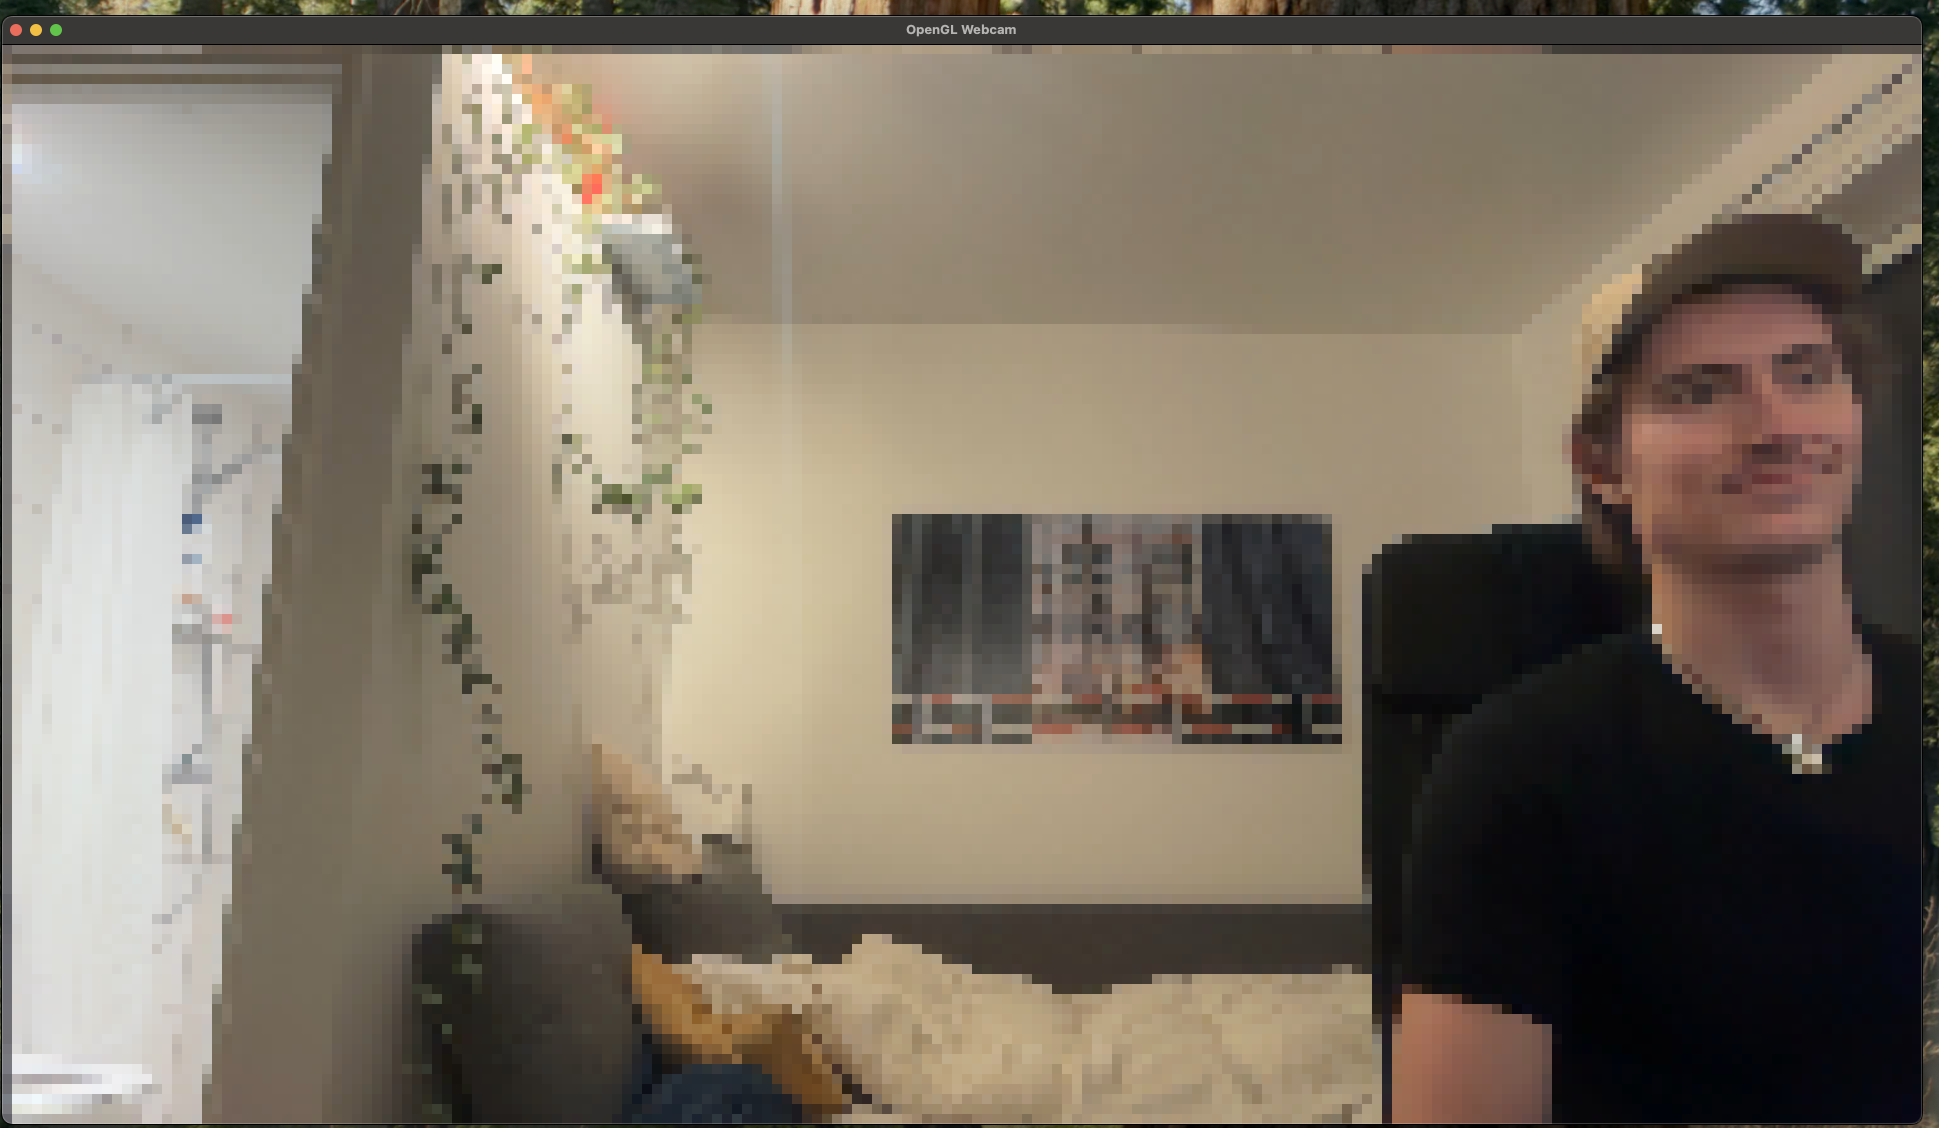
\includegraphics[width=\textwidth]{filters/pixelatio.png}
        \caption{Pixelation (10×10 blocks)}
        \label{fig:filter_pixelation}
    \end{subfigure}
    \hfill
    \begin{subfigure}[b]{0.20\textwidth}
        \centering
        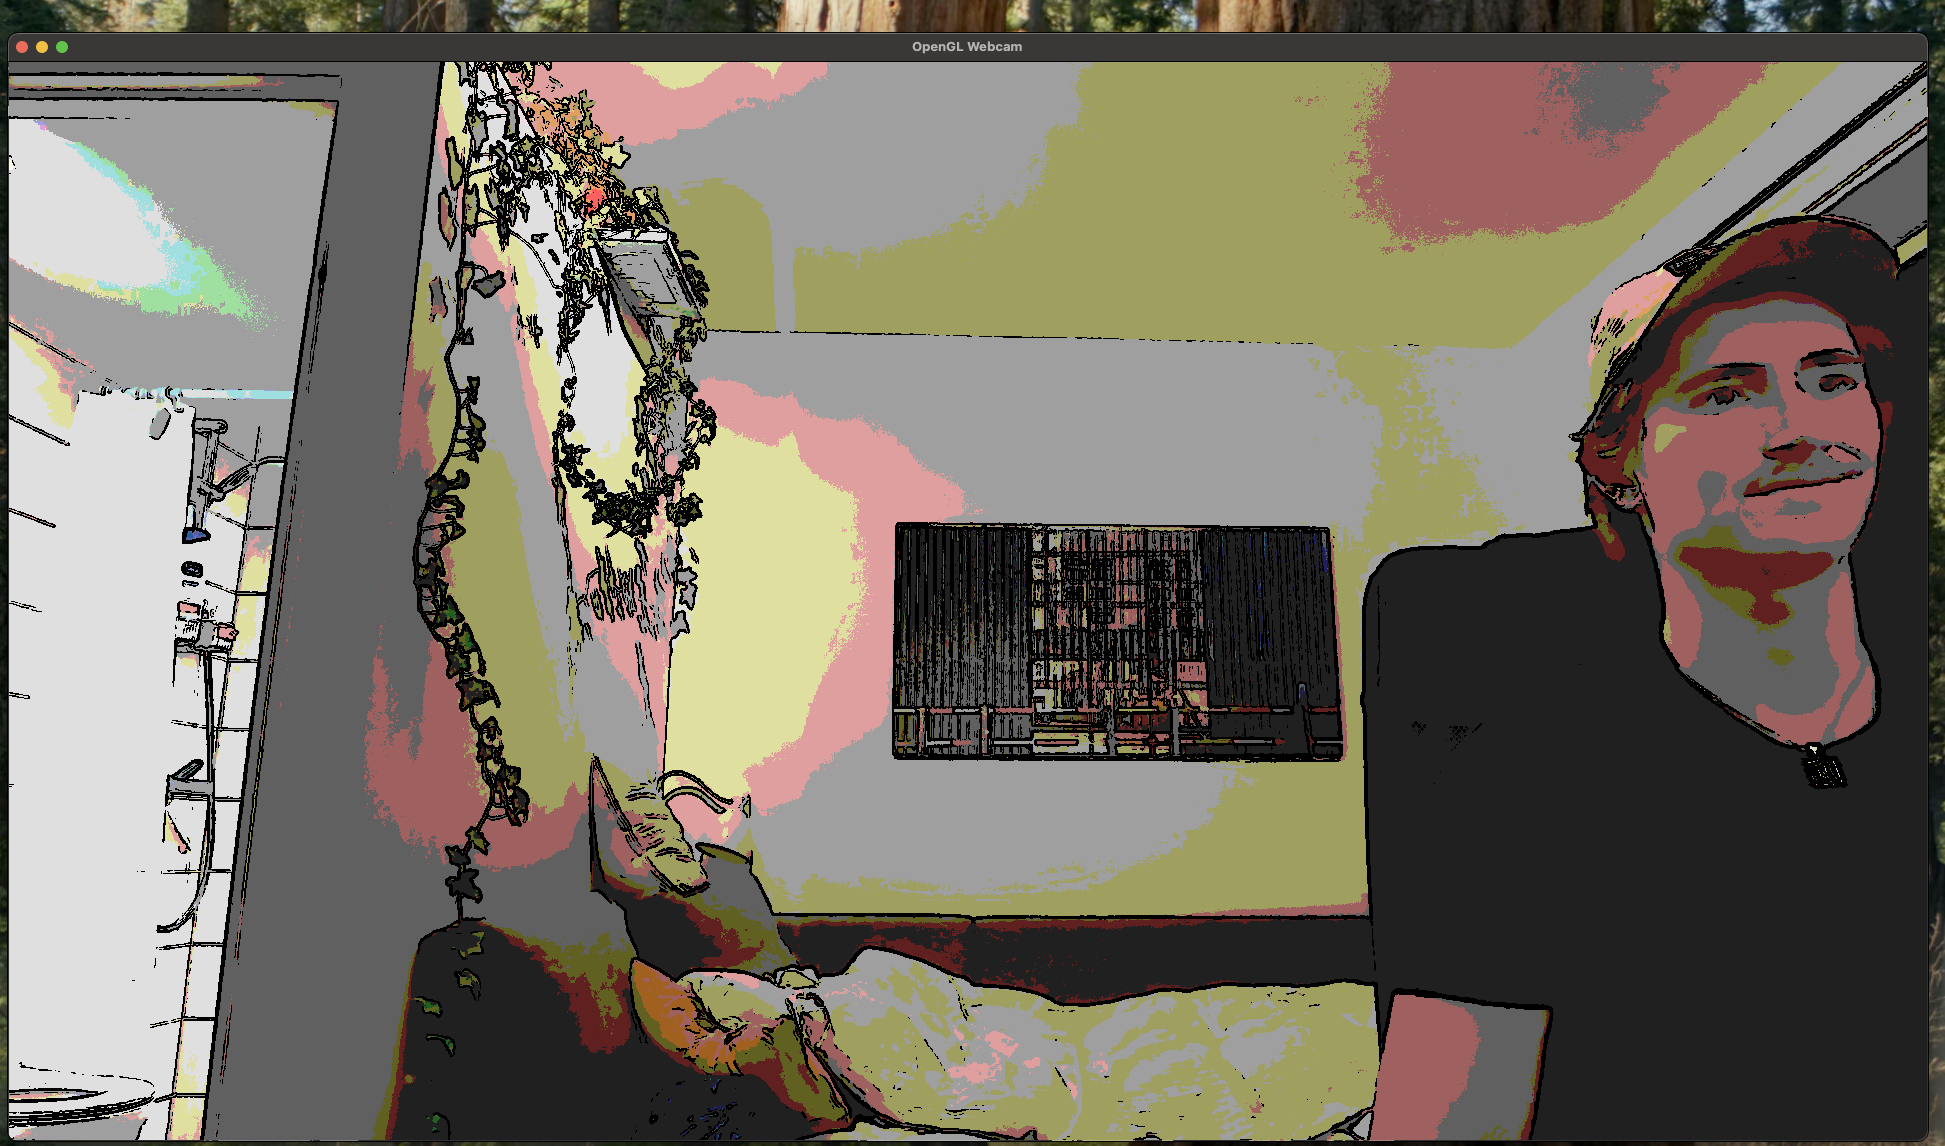
\includegraphics[width=\textwidth]{filters/comic.png}
        \caption{Comic Art}
        \label{fig:filter_comic}
    \end{subfigure}

    \caption{Visual comparison of implemented filters. (a) Grayscale conversion reduces color information. (b) Gaussian blur creates smoothing effect. (c) Edge detection highlights contours using Sobel operator. (d) Pixelation creates blocky mosaic effect. (e) Comic art combines edge detection with color quantization for artistic effect.}
    \label{fig:filter_comparison}
\end{figure}


\end{document}